\documentclass{report}
\usepackage{hyperref}
\usepackage[ngerman]{babel}
\usepackage{amsmath}
\usepackage{amsfonts}
\usepackage{amsthm}
\usepackage{tcolorbox}
\usepackage[a4paper, total={7in, 9in}]{geometry}
\usepackage[font={scriptsize,it}]{caption}
\usepackage{scrextend}
\usepackage{graphicx}
\usepackage{caption}
\usepackage{subcaption}
\usepackage[utf8]{inputenc}
\usepackage[T1]{fontenc}
\DeclareUnicodeCharacter{2212}{-}
\usepackage{verbatim}
\usepackage{tikz}

\tikzset{
  treenode/.style = {shape=rectangle, rounded corners,
                     draw, align=center,
                     top color=white, bottom color=blue!20},
  root/.style     = {treenode, font=\Large, bottom color=red!30},
  env/.style      = {treenode, font=\ttfamily\normalsize},
  dummy/.style    = {circle,draw}
}

\tikzstyle{level 1}=[level distance=3.5cm, sibling distance=3.5cm]
\tikzstyle{level 2}=[level distance=3.5cm, sibling distance=2cm]

% floating figure for column
\newenvironment{Figure}
	{\par\medskip\noindent\minipage{\linewidth}}
	{\endminipage\par\medskip}

\theoremstyle{definition}
\newtheorem{definition}{Definition}

\theoremstyle{example}
\newtheorem*{example}{Example}

\begin{document}

\begin{titlepage}
   \vspace*{\stretch{1.0}}
   \begin{center}
      \Large\textbf{Information Engineering 1 - HS20}\\
      \large\textit{Pascal Brunner - brunnpa7}
   \end{center}
   \vspace*{\stretch{2.0}}
\end{titlepage}

% Beispiel Bild
%\begin{Figure}
%   \centering
%    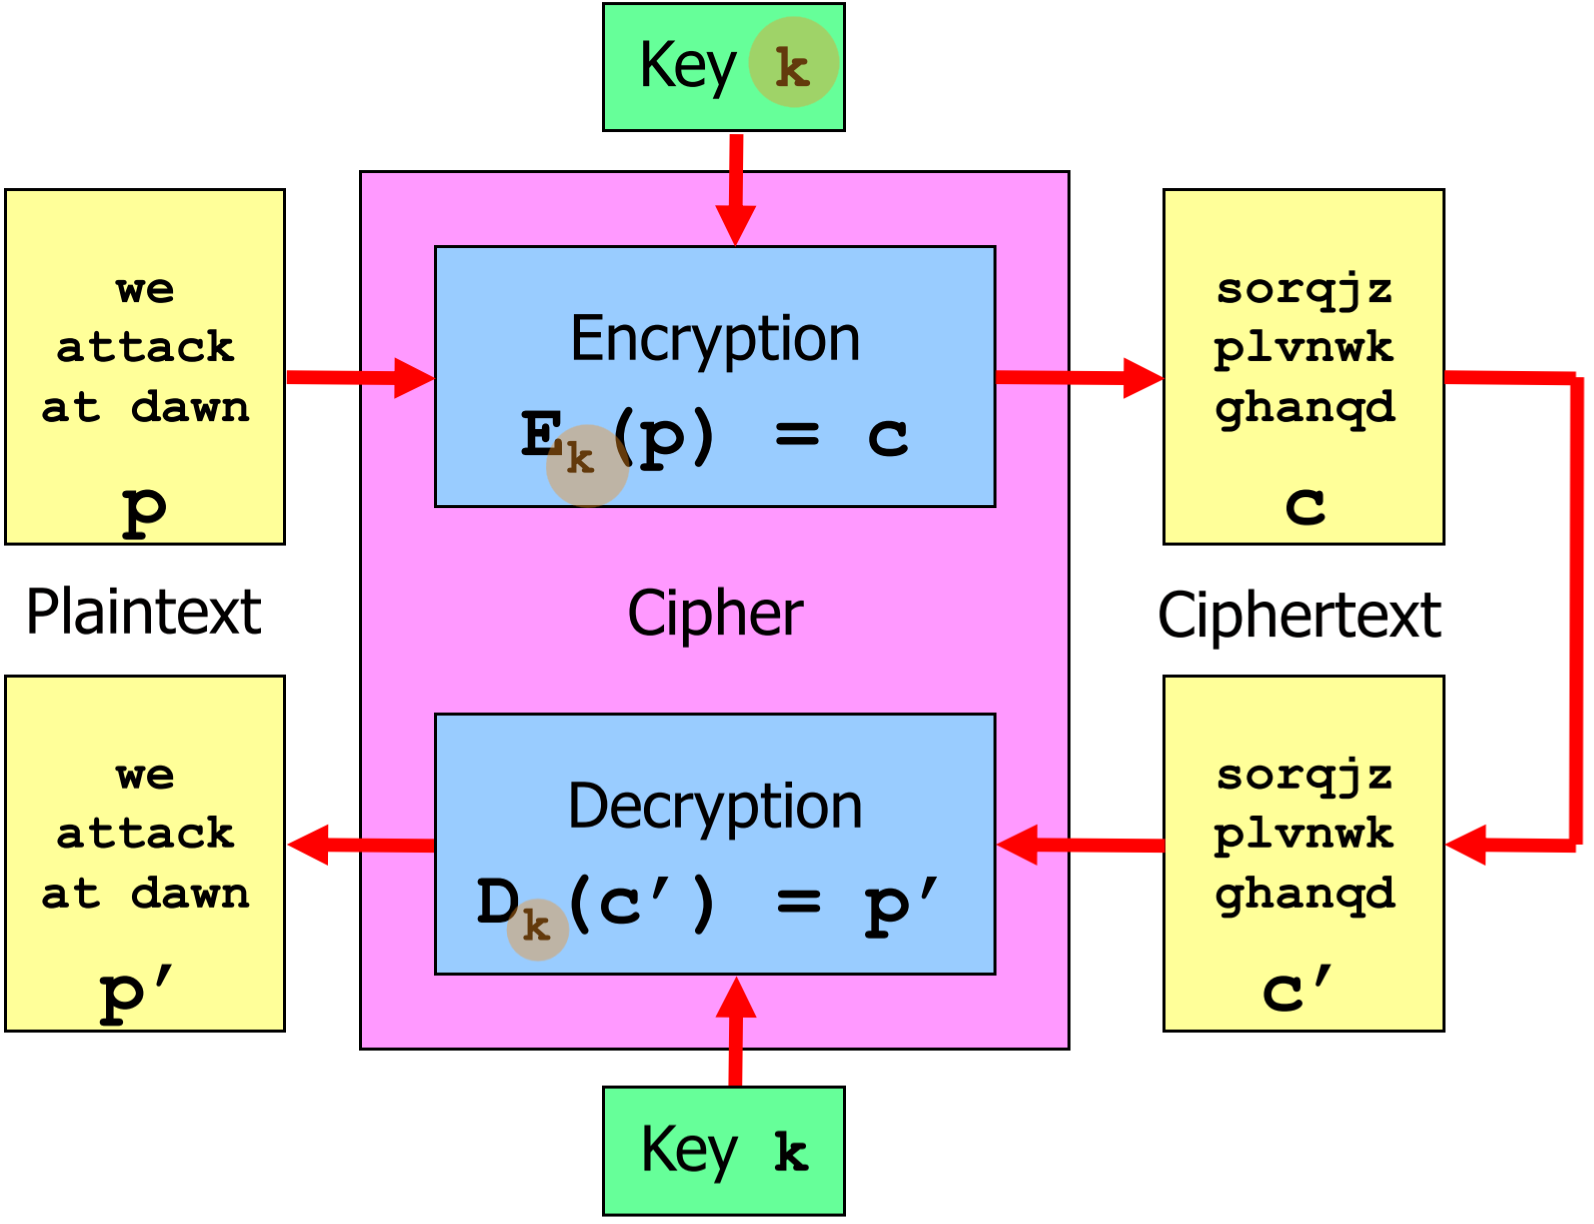
\includegraphics[width=150px]{img/BasicTerminologySecKeyCrypto.png}
%        \captionof{figure}{Basic Terminology basierend auf Secret Key Cryptography}
%        \label{fig:Basic Terminology}
%    \end{Figure}

\tableofcontents

\newpage

\chapter{Einführung}


\section{Information Retrieval - Definition}
\begin{itemize}
   \item Das akademische Fachgebiet, welches Methoden untersucht, um grosse Mengen an unstrukturierter und strukturierter information zu organisieren und bedürfnisgerecht aufzufinden
   \item Zugriff erfoglt im Allgemeinen in Form einer Anfrage (drückt Informationsbedürfnis mehr oder weniger treffend aus)
   \item Resultat im Allgemeinen in Form einer Rangliste von Dokumenten, (die gesuchte Information potentiell enthält)
\end{itemize}
$\Rightarrow$ Information Retrieval wird oft mit Retrieval auf unstrukturiertem Volltext in der Form von natürlichsprachigen Dokumenten gleichgesetzt.
Es werden fortgeschrittene Indexierungs- und Gewichtungsmethoden verwendet.

\subsection{Begriffsklärung}
Was ist der Unterschied zwischen Daten, Informationen, Wissen?\\
\textit{Daten}
\begin{itemize}
   \item Daten sind Codes
   \item Daten sind Symbole ohne keinen Kontext
   \item Fakten in einer codierten Form
   \item Daten tragen per se keine Bedeutung
   \item Daten sind in einem bestimmten Format (bspw. RTF, XML, JPEG)
   \item Daten können falsch oder korrekt sein (bspw. falsche Datenerfassung)
\end{itemize}

\textit{Informationen}
\begin{itemize}
   \item Daten werden interpretiert $\rightarrow$ Information
   \item Daten plus die Bedeutung, die ihnen beigemessen wird
   \item Information ist relevant oder irrelevant
   \item Information ist immer an ein Informationsbedürfnis gebunden
   \item Information benötigt man, um Aufgaben zu erledigen
   \item wird mit Hilfe von Daten dargestellt
   \item ist bzgl. einer Aufgabe mehr oder weniger relevant
   \item ist bzgl. einer Aufgabe mehr oder weniger vollständig
\end{itemize}

\textit{Wissen}
\begin{itemize}
   \item Das Resultat der Verarbeitung von Information (Schlüsse, Erkenntnisse)
   \item Wissen ist vernetzte Information (bspw. Geschäftsprozess)
   \item Häufig müssen interne und externe Informationen vernetzt werden
   \item Beispiele
   \subitem Bestellung eines Kunden abwickeln
   \subitem Flugzeug warten
   \subitem Marketing-Strategie entwickeln 
\end{itemize}

\subsection{Was ist das Ziel eines Information-Retrieval Systems sein?}
\begin{itemize}
   \item Retrievalproblem: \textit{Das Auffinden von möglichst viel relevanter Information 
   bei gleichzeitigem Minimieren der ebenfalls gelieferten irrelevanten Informationen}
   \item Wir wollen nicht nur Informationen wieder finden, sondern vor allem neue Informationen finden. 
   Die Information wird indirekt geliefert, in Form von relevanten Dokumenten
\end{itemize}

\section{Das Retrievalproblem}

\begin{itemize}
   \item Sprache ist nicht \textit{eindeutig} (Synonym, Homonyme, Metaphern, Schreibfehler etc.) 
   \item Informationsbedürfnisse werden ungenügend verbalisiert
   \item Informationsbedürfnisse werden ungenügend formuliert
   \item Die Dokumente und Informationen im System sind unstrukturiert oder inhomogen
   \item Irreführender Inhalt
   \item Autorität, Quelle, Aktualität, Urheberrecht, Einsammeln der Dokumente
   \item Widersprüchliche Ziele $\rightarrow$ Ausbeute vs. Präzision
\end{itemize}

Typische Annahmen für Volltextsuche:
\begin{itemize}
   \item Benutzer sucht relevante Elemente
   \item Benutzer kennt das gesuchte Elemente nicht
   \item Anzahl der relevante Elemente ist unbekannt
\end{itemize}

Der Begriff \textbf{Relevanz} ist wichtig für Information Engineering.\\
Das Verständnis einer Anfrage und eines Dokuments hängt immer auch vom konkreten Benutzer ab. \\
$\Rightarrow$ Das gelieferte Resultat ist nicht für jeden Benutzer gleich relevant.

\subsection{Konsequenzen des Retrievalproblems}
Der 'unscharfe' Begriff der relevanz und die vielfältige Darstellungsformen der Information, welche eine Übereinstimmung von Anfragen und Dokument erschweren,
führen zu einer wahrscheinlichkeitsbasierten Lösung:
\begin{itemize}
   \item Es werden diejenigen Dokumente geliefert, für welche die Wahrscheinlichkeit, dass sie vom Benutzer als relevant zur Anfrage beurteilt werden, am höchsten sind
   \item Ein Retrievalresultat ist fast nie vollständig 'korrekt': Es fehlen relevante Dokumente, oder irrelevante Dokumente werden zusätzlich gefunden
   \item Merke: 'scharfe Kriterien' (ja / nein) sind ungeeignet, da der Benutzer die Anzahl und die Form der gesuchten Dokumente kennen müsste, um eine Anfrage zu formulieren, welche das gewünschte Resultat liefer $\rightarrow$ Paradox
\end{itemize}

\subsection{IR Prozess}

\begin{enumerate}
   \item Man braucht eine gewisse Information
   \item In einem ersten Schritt möchte man eine Verbalisierung vornehmen $\rightarrow$ Ich brauche einen gute CD-Brenner
   \item Das ganze wird auf ein paar Stichworte hinuntergebrochen $\rightarrow$ CD-Brenner
   \item Das System muss nun eine Rangliste zusammenstellen, welche aufgrund der Anfrage geführt werden $\rightarrow$ Retrieval
   \subitem In diesem Prozess liegt die eigentliche Power von Information Engineering von Informationsbedürfniss-Formulierung zur Rangliste 
   \item Man erhält das Resultat in Form einer Rangliste $\rightarrow$ Die Relevanz folgt aus dem eigentlichen Informationsbedürfnis 
   \subitem Das System muss aus einer schlecht formulierten Informationsbedürfnis, ein möglichst gutes Ergebnis erhalten  
\end{enumerate}

\begin{Figure}
   \centering
    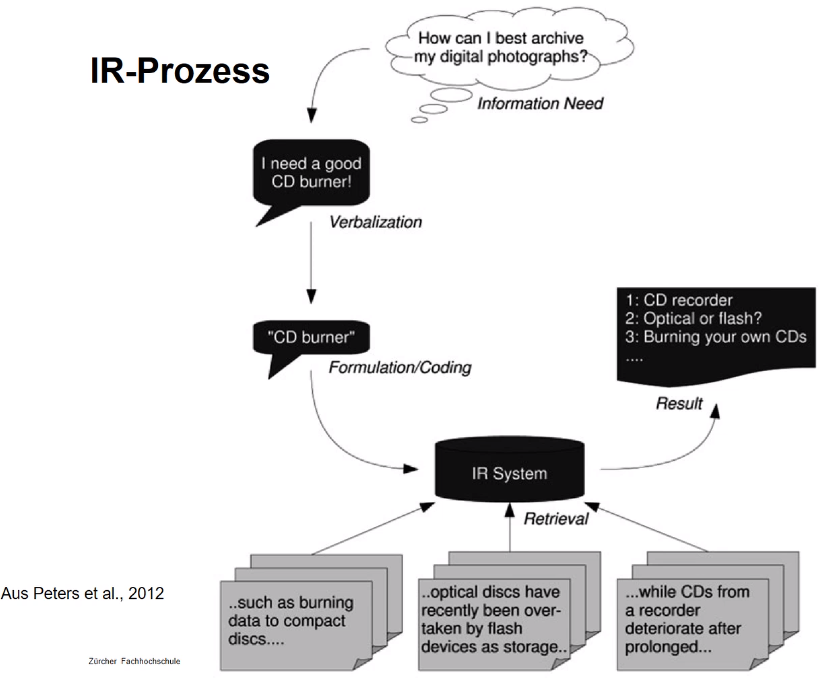
\includegraphics[width=150px]{img/IRProzess.png}
        \captionof{figure}{Ablauf eines Informationretrieval-Prozesses}
        \label{fig:IR Process}
\end{Figure}

\subsection{Verbalisierung / Codierung}
\begin{itemize}
   \item Verbalisierung Verstehen des Problems $\rightarrow$ richtige Begriff, Vollständigkeit
   \subitem Paradox: Muss Problem verstanden haben, um es richtig zu verbalisieren
   \item Codierung Verstehen des Systems $\rightarrow$ richtige Operatoren etc.
   \subitem Paradox: muss die Resultate kennen, um Anfragen richtig zu codieren 
   \item Das System kann a priori nur die explizite Information, welche in der 'codierten' Anfrage enthalten ist, auswerten.
   \item Das Resultat bevorzugt also Entscheide, welche bestmöglich zu dieser 'codierten Anfrage' passen. Nicht explizit formulierte Präferenzen oder Hintergrundwissen des
   Benutzers können nicht in die Resultatfindung einfliessen.
   \item $\Rightarrow$ Das Resultat ist immer nur so gut wie die Anfrage
\end{itemize}

\section{Das Suchparadox}
\begin{itemize}
   \item Google kann sich Vereinfachungen erlauben dank dem Suchparadox
   \item Es ist einfacher, in mehreren Milliarden Dokumenten zu suchen als in mehreren Tausend
   \item Wird auf kleinen Datenmenge gesucht, so ist eine Übereinstimmung zwischen Informationsbedürfnis und Dokumente schwerer nachzuweisen
\end{itemize}

   \subsection{Vom Informationsbedürfnis zur Information}
\begin{itemize}
   \item Der 'Bibliothekar' hilft dem Benutzer das Informationsbedürfnis zu verbalisieren und in eine Form zu bringen, um nach den gewünschten Information suchen zu können
   \item Hilft gegebenfalls auch, das Informationsbedürfnisbesser zu verstehen
   \item $\Rightarrow$ IR-Systeme können ähnliche Funktionen übernehmen
   \item Informationelle, navigationale, transaktionale, örtlich gebundene Bedürfnisse
\end{itemize}

\section{Information Retrieval Paradigmen}
\begin{itemize}
   \item Pull: Aufgrund eines Ad-hoc Informationsbedürfnisses Dokumente mit relevanten Informationen suchen
   \subitem Google Suche 
   \item Push: Dokumente mit relevanten Informationen aus einem Dokumentenstrom herausfiltern und weiterleiten
   \subitem Bspw. Mail von Netflix wenn neue Serie auf den Markt kommt wo mir gefallen könnte
   \item Browse: Neue Dokumente kategrorisieren und in eine Informationsstruktur einordnen 
\end{itemize}

\subsection{Ad-hoc Suche PULL}
Beispiele:
\begin{itemize}
   \item Suche des Bundesgerichtes
   \item Google Suche
\end{itemize}

\begin{Figure}
   \centering
    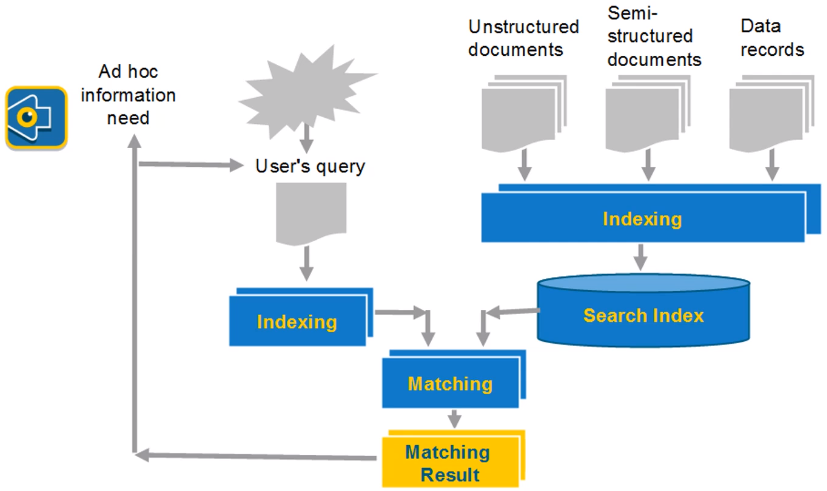
\includegraphics[width=150px]{img/PullParadigma.png}
        \captionof{figure}{Ablauf eines der Ad-hoc Suche}
        \label{fig:Ablauf Ad-hoc Suche}
\end{Figure}

\subsection{Bringdienste PUSH}
\begin{itemize}
   \item Das User-Profil dient für die Langlebigkeit
   \subitem Instagram sammeln der Likes, Bewertung von Filmen auf Netflix 
\end{itemize}

\begin{Figure}
   \centering
    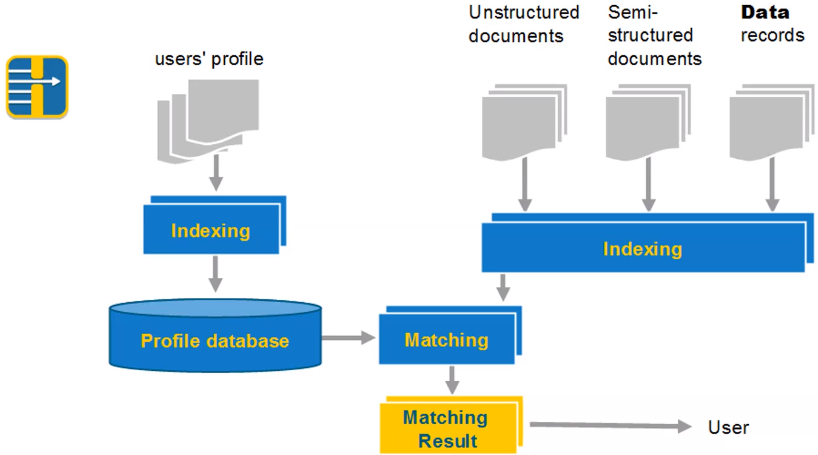
\includegraphics[width=150px]{img/PushParadigma.png}
        \captionof{figure}{Ablauf eines der Bringdienste}
        \label{fig:Ablauf Bringdienste}
\end{Figure}

\subsection{Browsing}
Beispiel
\begin{itemize}
   \item Ehemals Yahoo $\rightarrow$ War das Telefonbuch des Internets mit den diversen Links
\end{itemize}

\begin{Figure}
   \centering
    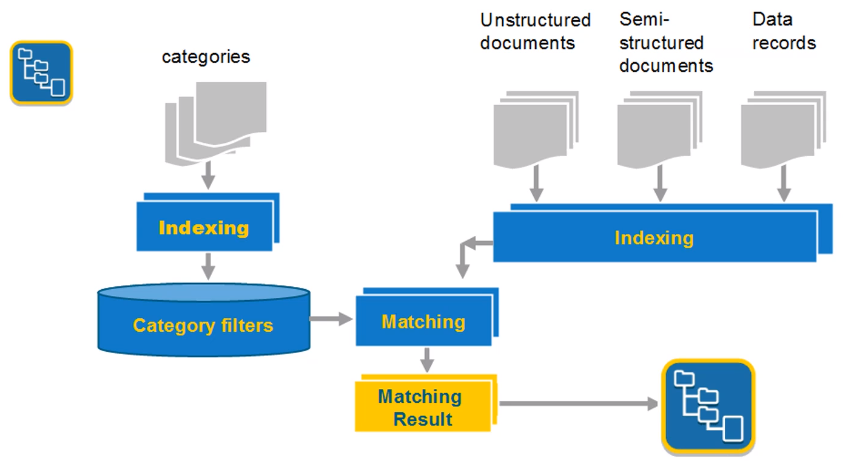
\includegraphics[width=150px]{img/BrowseParadigma.png}
        \captionof{figure}{Ablauf des Browsings}
        \label{fig:Ablauf Browse}
\end{Figure}

\section{Datenbank vs. IR}
Datenbank = strukturiert, exact-match (passt oder nicht)
IR = unstrukturiert, best-match (rangliste)

\begin{itemize}
   \item DB liefern für strukturierte Daten mit kontrolliertem Vokabular perfekte Resultate
   \item Daten in DB sollten unabhängig sein von der Applikation. Redundanz wird vermieden
   \item Elemente sind entweder Teil der Resultatmenge oder nicht
   \item Boole'sche Kriterien zur Selektion
   \item Geeignet für die Suche in (hoch-)strukturierter Information mit kontrolliertem Vokabular
\end{itemize}

\begin{Figure}
   \centering
    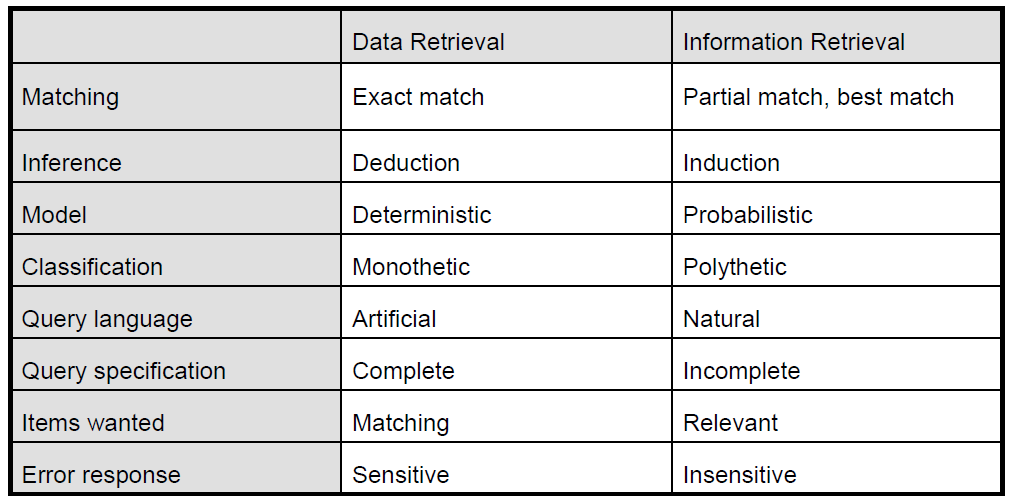
\includegraphics[width=150px]{img/IRvsDB.png}
        \captionof{figure}{Unterschied von IR vs DB}
        \label{fig:Unterschied von IR vs DB}
\end{Figure}

\section{Masse für Retrieval Effektivität}
Jedes IR-System liefert unterschiedliche Resultate
\begin{itemize}
   \item Retrievalresultate sind fast nie perfekt. Es sind Masse nötig, um die Qualität eines Retrieval Resultats zu beurteilen
   \item Zwei allgemein anerkannte Masse für Retrieval Qualität sind \textbf{Ausbeute} und \textbf{Präzision}
   \item Diese Eigenschaften dieser Masse sind gut analysiert und verstanden
   \item Beide Masse modellieren die Annahme, dass möglichst viel relevante und möglichst wenig irrelevante Information gefunden werden
\end{itemize}

\begin{equation}
   \text{Präzision} := \frac{\text{Anzahl relevante Dokumente im Resultat}}{\text{Anzahl Dokumente im Resultat}}
\end{equation}

\begin{equation}
   \text{Ausbeute} := \frac{\text{Anzahl Dokumente im Resultat}}{\text{Anzahl relevante Dokumente in der Kollektion}}
\end{equation}
$\rightarrow$ Ziel: Optimierung eines oder beider Kriterien\\

\begin{Figure}
   \centering
    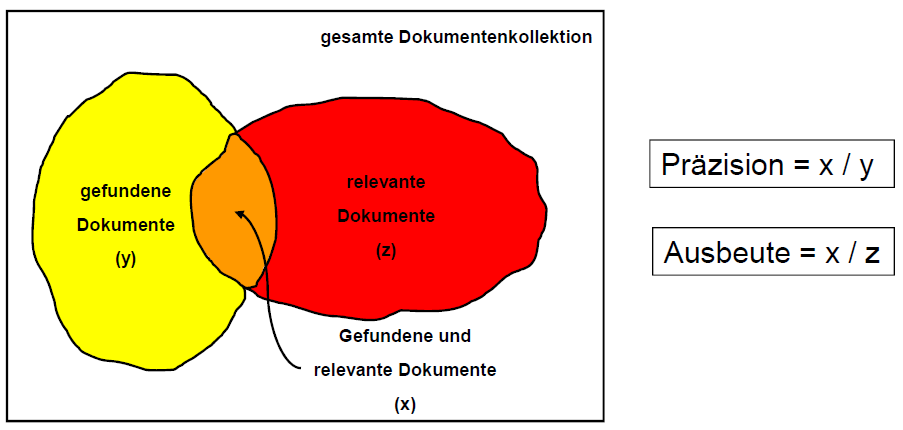
\includegraphics[width=150px]{img/AusbeutePraezision.png}
        \captionof{figure}{Visualisierung der Messgrössen}
        \label{fig:Visualisierung der Messgroessen}
\end{Figure}

\begin{Figure}
   \centering
    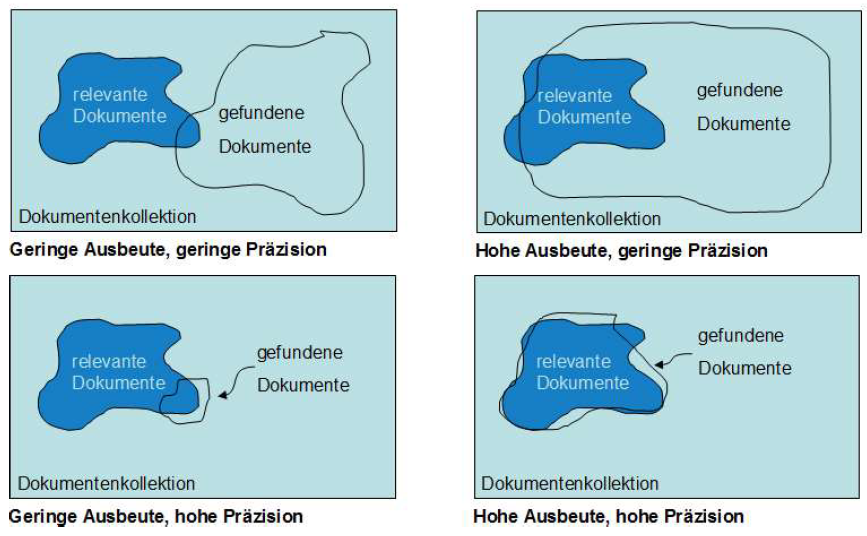
\includegraphics[width=150px]{img/AusbeutePraezisionSzenarien.png}
        \captionof{figure}{Szenarien der Messgrössen}
        \label{fig:Szenarien der Messgroessen}
\end{Figure}

\subsection{Probability Ranking Principle}
Eine Anordnung der gefundenen Dokumente in der Reihenfolge ihrer Wahrscheinlichkeit, dass sie zur Anfrage relevant sind
unter Berücksichtigung sämtlicher zur Verfügung stehender Informationen und geeigneter Annahmen, ist optimal in mehrerer Hinsicht.\\
Falls das sogenannte Probability Ranking Principle befolgt wird, lassen sich die folgende Eigenschaften mathematisch beweisen
\begin{itemize}
   \item Die Präzision an einem beliebigen 'cut-off-point' wird optimiert
   \item Die Ausbeute an einem beliebigen 'cut-off-point' wird optimiert
   \item Die Kosten der Auswertung (relevant = positiv, irrelevant = negativ) werden optimiert
\end{itemize}

$\Rightarrow$ Die Verwendung von wahrscheinlichkeitsbasierten Ranglisten ist theoretisch fundiert

\chapter{Indexierung und Vergleich}
\section{Ausgangslage}
\begin{itemize}
   \item 1 vages Informationsbedürfnis
   \item 1'000'000 unstrukturierte Volltexte
   \item Gesucht $\rightarrow$ Resultat
   \item Vorgehen
   \subitem 1. Anfrage und Dokumente vergleichbar machen
   \subitem 2. Vergleich
   \item Datenbank vs. IR
   \subitem Datenbank: in Tabelle Apfel sind nur Äpfel
   \subitem IR: Es werden Apfel mit Birnen verglichen
\end{itemize}

\subsection{Was ist so schwierig?}
\begin{itemize}
   \item Sprache ist nicht eindeutig
   \subitem Synonyme, Homonyme, Umschreibungen, Metaphern etc.
   \item Bedeutung und Relevanz ändern mit der Zeit
   \subitem \textit{nine eleven}: Notfallnummer oder Inbegriff einer Zeitwende? oder doch ein Porsche?
   \item Menschen lernen dazu oder vergessen
   \item Sprache Akronyme, Phrasen, Komposita, verschiedene Schreibweisen
   \item Unschärfe macht uns das Leben schwer (im Retrieval, automatische Sprachverbreitung)
\end{itemize}



\section{Indexierung}

\subsection{Worthäufigkeit}
\begin{itemize}
   \item Worthäufigkeiten sind nicht gleich verteilt
   \item sehr viele Wörter sind sehr selten
\end{itemize}
\textbf{Zipfsches Gesetz}: Rang der Häufigkeit * Häufigkeit = konstant

\subsection{Anfrage und Dokument vergleichen}
Anfrage und Dokument können nicht direkt verglichen werden. Anfragen und Dokument müssen zuerst vergleichbar gemacht werden

\subsection{Verschlagwortung}
\begin{itemize}
   \item manuell, automatisch oder beides passieren
   \item Deskriptoren stammen aus einem Vokabular (freie Indexierung) oder aus einer autorisierten Liste (kontrollierte Indexierung)
   \item Zu beachten gilt
   \subitem Dokumentevokabular $\neq$ Anfragevokabular
   \subitem Manuelle Indexierung sehr aufwendig und kostspielig
\end{itemize}

\textbf{Automatische Verschlagwortung}\\
Ist nicht so einfach wie man einfach glauben kann


\subsection{Volltextindexierung}
Sondernfall von automatischer Verschlagwortung mit freiem Vokabular\\
\textbf{erschliessen}:
\begin{enumerate}
   \item Buchstabenumwandlung
   \item Wortextraktion
   \item Stoppwortelimination
\end{enumerate}

\subsubsection{Tokenisierung}
\begin{itemize}
   \item Tokenisierung (Wortextraktion) ist der Prozess der die einzelnen Wörter aus dem Text extrahiert
   \item Im Allgemeine werden einige oder alle der folgen Schritte ausgeführt
   \subitem Dokumentformate konvertieren
   \subitem Zeichencodierung anpassen
   \subitem Gross / Kleinschreibung normalisieren
   \subitem Text entlang Trennzeichen in Tokens separieren (eigentliche Tokenisierung)
   \item Letzte Punkt ist heikel (bspw. Hans Peter ein oder zwei Wörter) 
\end{itemize}

\subsubsection{Stoppwortelimination}
\begin{itemize}
   \item Häufigsten Wörter werden aus dem Text eliminiert
   \item Diese Wörter sind nicht inhaltstragend
   \item Treffer auf diesem Wörter sind (meist!) nicht hilfreich, und verdecken echte, wertvolle Treffer
   \item Stoppwörter machen etwa 40 \% des Textes aus
\end{itemize}

\textbf{Erschliessen}
\begin{itemize}
   \item Wortzerlegung
   \item Wortnormalisierung
\end{itemize}

\textbf{Stemming / Wortnormalisierung}
\begin{itemize}
   \item In Sprachen werden mehr oder weniger Wortformen verwendet, um Dinge wie Kasus, Numerus, Genus etc. anzuzeigen
   \item Dieses Phänomen ist je nach Sprache unterschiedlich stark ausgeprägt
   \subitem Im Englischen gibt es relativ wenig verschiedene Formen für die meisten Wörter
   \subitem Im Deutschen sieht das schon anders aus (bis zu 144 Formen für ein Verb) 
   \item Information Retrieval ist kein linguistischer Schönheitswettbewerb
   \item Wir wollen Dokumente auffinden unabhängig von einzelnen Wortformen
   \item Aber: Die Dokumente sollten relevant sein, d.h. der gesuchte Sachverhalt sollte abgebildet werden
   \item Wenn möglich werden im IR einfache, regelbasierte Verfahren verwendet, um die Wörter zu normalisieren
   \item Dieser \textit{Stemmer} produzieren teilweise unsinnige (abgeschnittene) wortformen, oder produzieren falsche Treffer $\rightarrow$ Frage der Gewichtung
\end{itemize}

\subsubsection{Komposita}
\begin{itemize}
   \item Im Deutschen können unendlich viele Komposita gebaut werden, indem man Wörter zusammengefügt
   \item Diese Komposita können nicht lexikalisch aufgezählt werden
   \item eigentlich sehr gute Suchbegriffe, aber: der gleiche Sachverhalt lässt sich immer auch als Nominalphrase umschreiben
   \item Es ist hilfreich solche Begriffe zu zerlegen (bis zu 30\% Effektivität-Gewinnung)
   \subitem jedoch sollte man bspw. \textit{Frühstück} nicht trennen 
\end{itemize}

\section{Bag of Words Modell}


\section{Rangierregeln}

\subsection{Rangierprinzipien}
\begin{itemize}
   \item Versuch "common sense" Regeln aufzustellen
   \item Es gibt KEINE konkreten Systeme, die diese Rangierprinzipien so implementieren, aber:
   \item Hilft bei späterer konkreter Umsetzung
   \item Hilft dem Benutzer als mentales Model
\end{itemize}

\textbf{Prinzip 1}\\
Je mehr Suchbegriffe (Terme) in einem Dokument vorkommen desto wahrscheinlicher ist das Dokument relevant\\

\textbf{Prinzip 2}\\
Je häufiger ein Suchbegriff in einem Dokument vorkommt, desto wahrscheinlicher ist das Dokument relevant $\rightarrow$ Merkmalshäufigkeit (Anzahl Vorkommen eines Merkmals in einem Dokument)\\

\textbf{Prinzip 3}\\
Dokumente, die seltene Suchbegriffe enthalten, sind mit höheren Wsk relevant als Dokument, die häufige Suchbegriffe enthalten $\rightarrow$ Dokumentenhäufigkeit (Anzahl Dokumente, die einen Begriff enthalten)\\

\textbf{Prinzip 4}\\
Je mehr Hyperlinks auf ein Dokument zeigen, desto wahrscheinlicher ist es relevant\\

\textbf{Prinzip 5}\\
Je näher die Suchbegriffe beieinander liegen desto relevanter das Dokument\\

\textbf{Prinzip 6}\\
Je früher die Suchbegriffe in einem Dokument vorkommen, desto höher seine Relevanz\\

\subsection{Wortstatistiken}
Zur Umsetzung der Rangierregeln sind eine Reihe von Statistiken notwendig:
\begin{itemize}
   \item tf - term frequency $\rightarrow$ Wie oft tritt ein Merkmal/Term in einem Dokument auf?
   \item df - document frequency $\rightarrow$ in wievielen Dokumenten tritt ein Merkmal/Term auf
   \item Dokumentlänge $\rightarrow$ ein Mass für die Länge des Dokuments bspw. Anzahl Tokens, Anzahl Merkmale, Bytelänge
   \item Position der Merkmale im Text, In-Links / Out-Links
\end{itemize}

\subsubsection{Inverse document frequncy}
\begin{itemize}
   \item $idf(\phi_k) = log(\frac{(1+N)}{1+df(\phi_k)})$
   \subitem N: Anzahl Dokumente in der Kollektion
   \subitem $df(\phi_k)$: Anzahl Dokumente die Term k erhalten
   \item Mit $idf(\phi_k)$ kann die Ausprägung (Wichtigkeit; wie 'charakteristisch') eines Terms für ein bestimmtes Dokument besser bestimmt werden als durch simples Zählen der Häufigkeit
   \item $w(\phi_k, d_i) = tf(\phi_k, d_i) * idf(\phi_k)$
   \subitem $tf(\phi_k,d_i)$: Anzahl des Vorkommen des Term k in Dokument i
   \subitem $idf(\phi_k)$: inverse Dokumentenhäufigkeit des Terms k
   \item $\Rightarrow$ Ein hohes Gewicht haben dabei Terme, die in wenigen Dokumenten innerhalb der Kollektion häufig auftreten
\end{itemize}

\subsection{Vektorraummodell}
\begin{itemize}
   \item Die Gewichtung einzelner Terme reicht nicht. Wir müssen die Anfragen als Ganzes mit dem Dokument als Ganzes vergleichen
   \item Fasse informationsobjekte $d_j$ und Anfrage $q$ als Vektoren im Merkmalsraum auf, jedes Merkmal $\rightarrow$ eine Dimension
   \item Vektor $dj = (\dots, w_{\phi_i}, \dots)$ (Gewicht $w_{\phi_i})$ bspw. 1 wenn das entsprechende Merkmal im Dokument ist, 0 sonst 
\end{itemize}

$\rightarrow$ Anfrage als Vektor, wobei Sim(Dokument, Anfrage) = Kosinus(Winkel)
\begin{Figure}
   \centering
    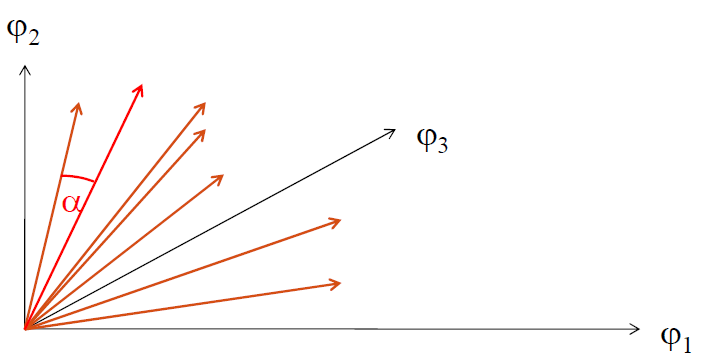
\includegraphics[width=300px]{img/Vektorraummodell.png}
        \captionof{figure}{Dokumente als Vektoren im n-dimensionalen Raum}
        \label{fig:Dokumente als Vektoren im n-dimensionalen Raum}
\end{Figure}

Problem: Merkmale spannen einen orthogonalen Raum auf. Merkmalabhängigkeiten passen nicht in das Modell. Das Modell liefert keine Antwort wie die einzelnen Merkmale zu gewichten sind\\
\textit{Bemerkung:} Zwei Vektoren heissen zueinander orthogonal, wenn ihr Skalarprodukt null ist.

\subsubsection{Längenormalisierung}
\begin{itemize}
   \item wenn Dokumente und Anfrage als Vektoren in einem n-dimensionalen Vektorraum dargestellt werden, hat sich folgende Gleichung als erfolgreich bewiesen
   \item $RSV = \frac{(q,d)}{||q|| ||d||} = cos(\alpha)$ $\rightarrow$ wobei RSV für \textit{retrieval status value} steht
   \subitem Winkel $\alpha$ ist der Winkel zwischen zwei Vektoren q und d
   \subitem (q,d) ist das skalare Produkte
   \subitem || || kennzeichnet die Länge des Vektors 
\end{itemize}

\subsubsection{Gewichtungsformel}
Es ergibt sich bei Kombination mit tf.idf-Gewichtung die folgende Gewichtungsformel (\textit{tf-idf-cosinus}):
\begin{eqnarray}
   \begin{split}
      a_{i,j} &:= ff(\phi_i, d_j) * idf(\phi_i)\\
      b_i &:= ff(\phi_i, q) * idf(\phi_i)\\
      RSV(q,d_j) &:= \frac{\sum_{\phi_i \in \Phi(q) \cap \Phi(d_j)} a_{i,j}*b_i}{\sqrt{\sum_{\phi_i \in \Phi(d_j)}a^2_{i,j}} * \sqrt{\sum_{\phi_i \in \Phi(q)}b^2_i}}
   \end{split}
\end{eqnarray}

\subsubsection{Relevanzrückkoppelung (englisch: relevance feedback)}
\textbf{Idee:} der/die BenutzerIn identifiziert im Resultat relevante und irrelevante Dokumente\\
Dabei wird ein neuer Vektor konstruiert, der näher bei den relevanten Dokumenten und weiter weg von den irrelevanten Dokumenten liegt
\begin{Figure}
   \centering
    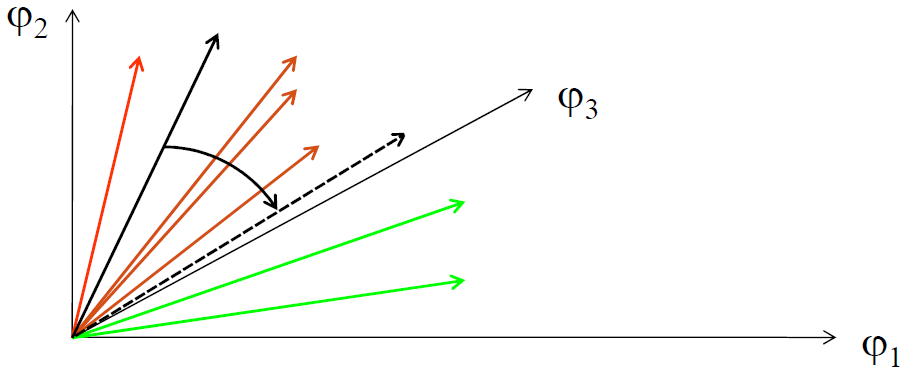
\includegraphics[width=150px]{img/relevanceFeedback.png}
        \captionof{figure}{neuer Vektor im relevance Feedback Prozess}
        \label{fig:neuer Vektor im relevance Feedback Prozess}
\end{Figure}

Dies kann man mit verschiedenen Spielarten realisieren:
\begin{itemize}
   \item Originalanfrage wird neu gewichtet
   \item Originalanfrage wird um neue Begriffe aus den relevanten Dokumenten ergänzt
   \item Kombination aus 1 und 2
   \item Eine komplett neue Anfrage wird nur aus den relevanten Dokumenten konstruiert
\end{itemize}

\begin{Figure}
   \centering
    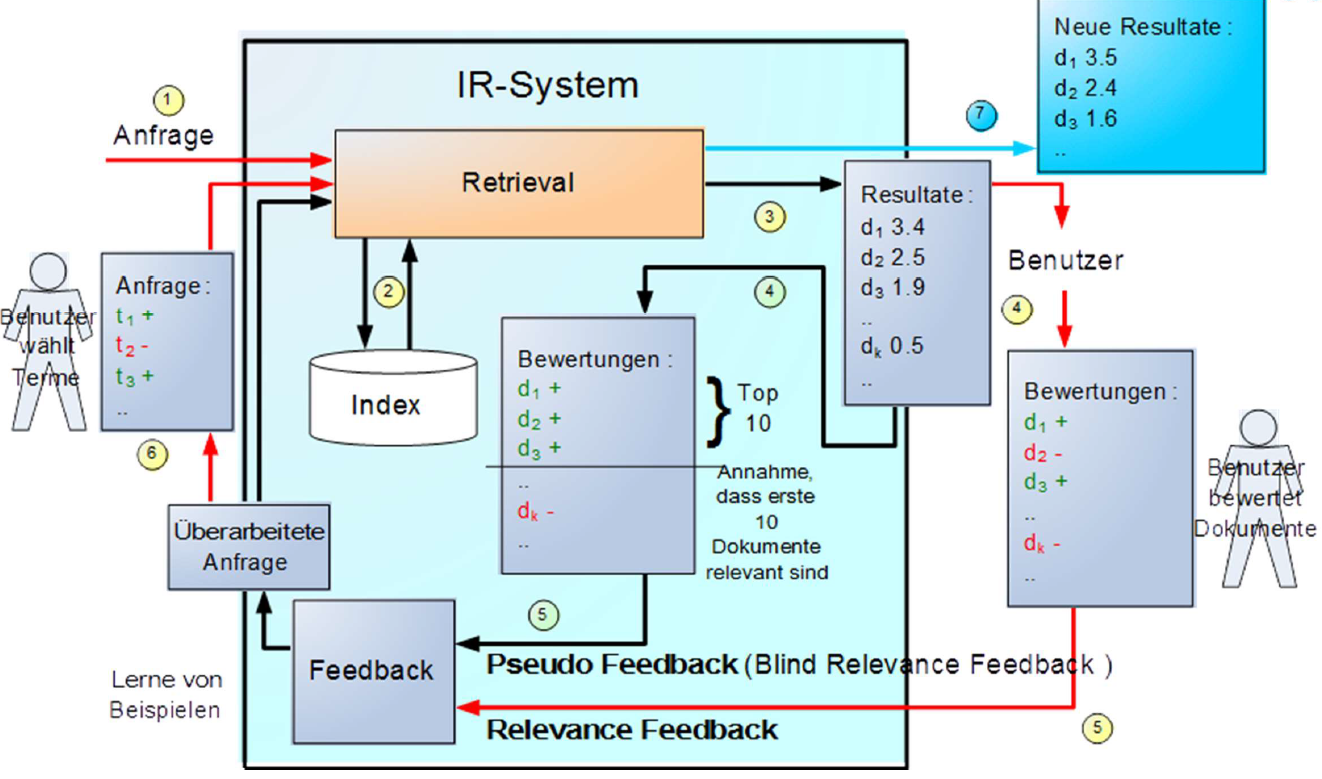
\includegraphics[width=150px]{img/schemaRelevanceFeedback.png}
        \captionof{figure}{Schema von relevance Feedback Prozess}
        \label{fig:Schema von relevance Feedback Prozess}
\end{Figure}

\subsection{Probability Ranking Principle}
\textit{If a reference retrieval system's response to each request is a ranking of the
documents in the collections in order of decreasing probability of usefulness to
the user who submitted the request, where the probabilities are estimated as
accurately as possible on the basis of whatever data has been made available
to the system for this purpose, then the overall effectiveness of the system to
its users will be the best that is obtainable on the basis of that data. (S.E.
Robertson, 1977)}

$\Rightarrow$ eigentlich geht es darum, dass man Systeme bauen, welche eine Rangliste zurückliefern in absteigender Wahrscheinlichkeit / Relevanz, dann ist das eine Optimale Strategie

\begin{itemize}
   \item PRP ist eher eine Hypothese als ein Prinzip
   \item \textit{will be the best}: Es gibt Rahmenbedingungen und Annahmen, z.b. Kosten für gefundene irrelevante Dokumente und Kosten für nicht gefundene relevante Dokumente, dann kann man beweisen. PRP minimiert die Erwartungskosten
   \item \textit{Estimated as accurately as possible}: hier liegt das Problem $\rightarrow$ wie schätzen wir diese Wahrscheinlichkeit ab?
\end{itemize}

\textbf{Beispiel:}
\begin{Figure}
   \centering
    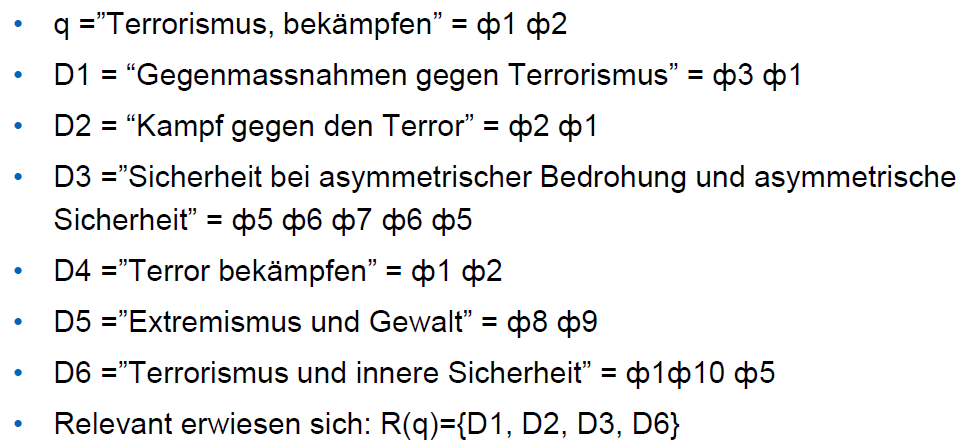
\includegraphics[width=150px]{img/BeispielPRP.png}
        \captionof{figure}{Beispiel eines PRP}
        \label{fig:Beispiel eines PRP}
\end{Figure}

\begin{Figure}
   \centering
    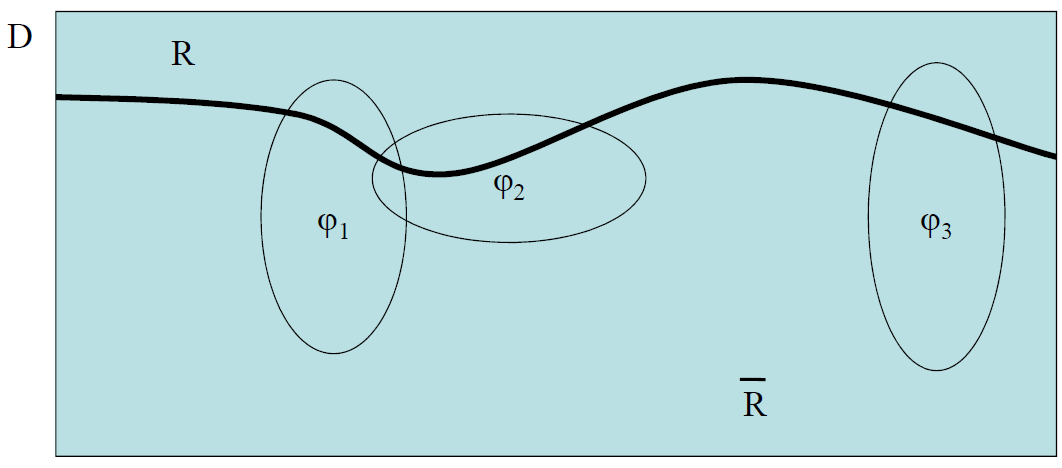
\includegraphics[width=150px]{img/BeispielVisualisiert.png}
        \captionof{figure}{Beispiel visualisiert eines PRP}
        \label{fig:Beispiel visualisiert eines PRP}
\end{Figure}

\section{Probabilistisches Retrieval}
\begin{itemize}
   \item Probabilistisches Retrieval: Eine Gruppe von verwandten Modellen, die die wahrscheinlichkeitstheoretische Auffasung des Retrievalsproblems zugrunde legen
   \item Anfänge frühe 60er Jahre
   \item Die Grenzen des Probabilistisches Retrievals scheinen erreicht zu sein
\end{itemize}

\subsection{Werkzeuge}
\begin{itemize}
   \item A, B stochastisch unabhängig, dann $P(A,B) = P(A)*P(B)$
   \item Bedingte Wahrscheinlichkeit: $P(A|B)=\frac{P(A,B)}{P(B)}$
   \item Bayes: $P(A|B) = \frac{P(A)P(B|A)}{P(B)}$
   \item DAS PRP fordert $RSV(q,d) = f(P(R|q,d)) + g(q)$ d.h. eine ordnungserhaltenede Funktion auf der Wahrscheinlichkeit, dass ein Dokument d zur Anfrage q als relevant betrachtet wird
   \subitem $\Rightarrow$ absolute Scores sind als für die Rangierung nicht wichtig 
\end{itemize}

\section{Boole'sches Retrieval}
Dabei handelt es sich um eines der ältesten Methoden (bspw. auch in Datenbanken). Dabei wird die Frage als Boolsche Ausdruck bzw. durch boolescher Logik die Abfrage evaluiert

\subsection{Anhaftende Probleme}
\begin{itemize}
   \item Das Resultat kann riesig sein, vor allem bei kurzen Anfragen (bspw. Bier) $\rightarrow$ Resultatmenge sind nicht nach Relevanz sortiert
   \item Kleine Anpassungen bei einer Anfrage kann zu sehr unterschiedlichen Resultatmengen führen $\rightarrow$ häufig zu gross oder zu klein
\end{itemize}

\subsection{Paradox}
Weil der Benutzer wenig Einfluss auf die Grösse der Resultatmenge hat (diese aber im Gegensatz zu wahrscheinlichkeitsbasierten Ranglisten wichtig ist), findet der Benutzer immer zuviel oder zuwenig $\rightarrow$ müsste das Resultat kennen um eine geeignete Anfrage zu stelleny


\chapter{Systeme und Architektur}
\iffalse

\begin{Figure}
   \centering
    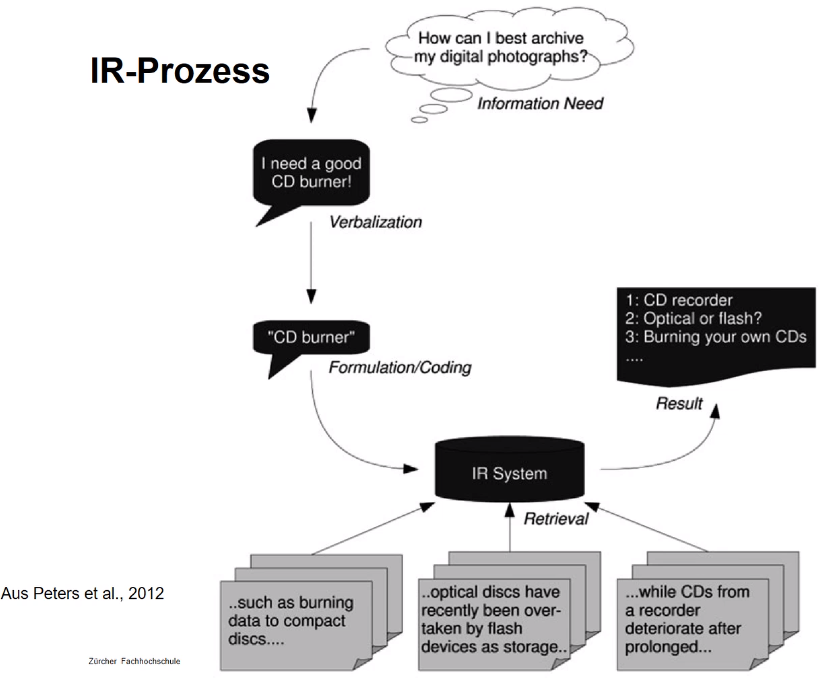
\includegraphics[width=150px]{img/IRProzess.png}
        \captionof{figure}{Ablauf eines Informationsretrieval-Prozesses}
        \label{fig:IR Process}
\end{Figure}
\fi

\section{Invertierte Liste}
Eine invertierte LIste besteht aus einer geordneten Liste von Merkmalen mit mindestens Information über die Häufigkeit jedes Merkmals in der Dokumentenkollektion

\begin{Figure}
   \centering
    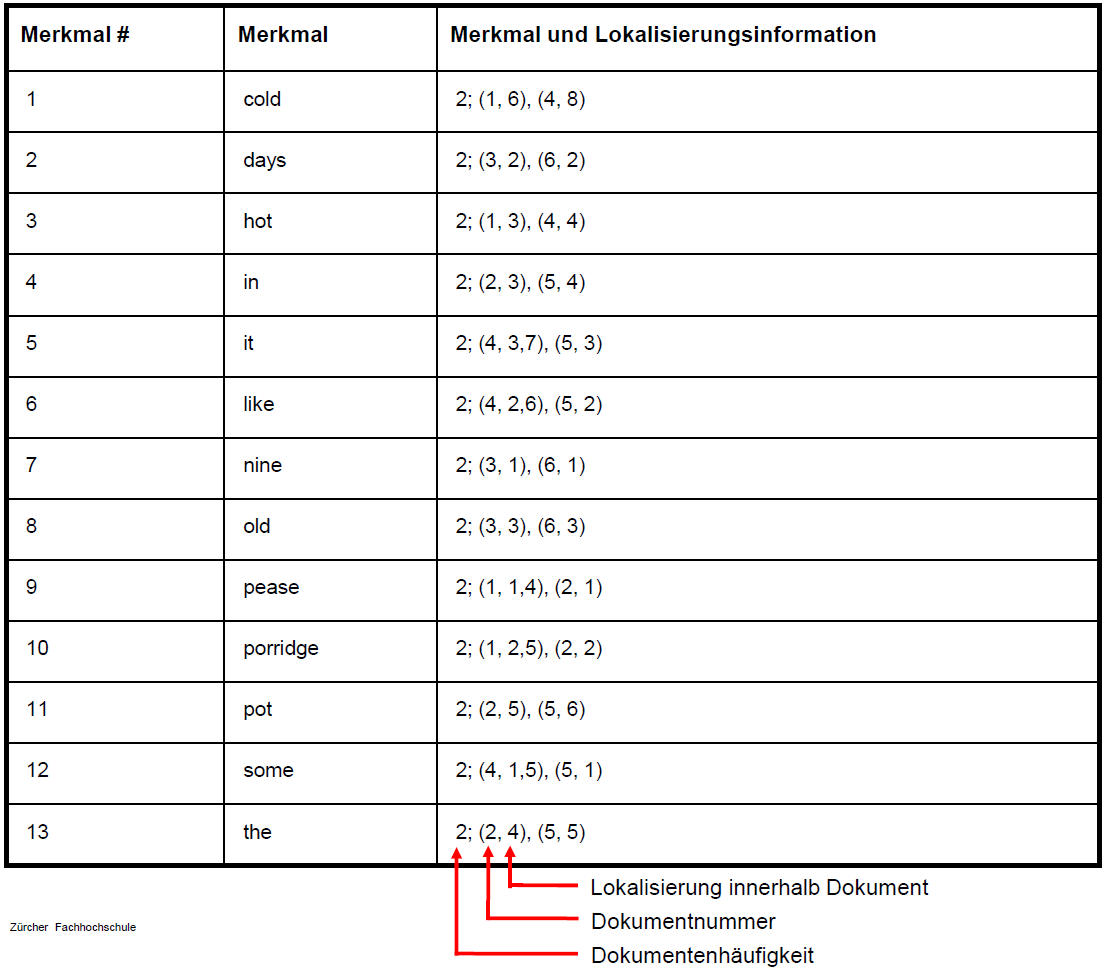
\includegraphics[width=150px]{img/invertierteListe.png}
        \captionof{figure}{Abbildung einer beispielhaften invertierten Liste}
        \label{fig:Abbildung einer beispielhaften invertierten Liste}
\end{Figure}

\subsection{Inhalt einer invertierten Liste}
\begin{itemize}
   \item invertierte Liste zeigt
   \subitem Dokumenthäufigkeit (bspw. in wie vielen Dokumenten ein Merkmal auftritt)
   \subitem in welchem Dokument das Merkmal auftritt
   \subitem an welcher Stelle im Dokument das Merkmal auftritt (optional)
   \item invertierte Liste kann mehr oder weniger Informationen enthalten
   \subitem Gewichtung der Merkmale
   \subitem Kategorisierung der Merkmale
\end{itemize}

\subsection{Granularität einer invertierten Liste}
$\rightarrow$ Ist die Genauigkeit, zu welcher eine invertierte Liste die Lokalisierung der Merkmale festlegt

\begin{itemize}
   \item Grober Index
   \subitem bspw. nur Blöcke von Texten in welchen mehrere Dokumente gespeichert sein können 
   \item Mittlerer Index
   \subitem bspw. die Lokalisierung sind als Dokumentennummern gespeichert 
   \item Feiner Index
   \subitem Index liefert ein Satz, Wort oder sogar Byte zurück 
\end{itemize}
$\rightarrow$ wir brauchen in etwa eine Grössenordnung des Index in Grösse des eigentlichen Dokumentes.

\subsection{Boolesches Retrieval mittels invertierter Liste}
Resultat wird aus der invertierten Liste generiert $\rightarrow$ durch and, or, oder not (wobei not, selten unterstützt ist)

\subsection{Lokalisierungsmerkmale in Listen}
Eine invertierte Liste ist eine extrem grosse Liste mit allen Merkmalen aus allen Dokumenten als Einträgen. Wenn Anfragen verarbeitet werden, müssen diese Merkmale aufgefunden werden:
\begin{itemize}
   \item Speichere die Merkmale in einer alphabetischen Liste $\rightarrow$ Durchlaufe die geordnete Liste $\Rightarrow$ $O(\log(n))$
   \item Speichere die Merkmale in einer Hash-Tabelle $\rightarrow$ Lokalisierung der Merkmale in einer Hash-Tabelle ist sehr schnell $\Rightarrow$ $O(1)$
\end{itemize}

\subsubsection{Hash-Datei}
\begin{itemize}
   \item Adressierung im Hash
   \item Die Hash-Funktion h erstellt Adressen, die zu den Merkmalen zeigen
   \item Idealerweise sollte die Hash-Funktion h die Adressen gleichmässig über den verfügbaren Speicherraum verteilen
   \item Idealerweise sollten zwei merkmal $t_i$ und $t_j$ die unterschiedlich sind ($t_i \neq t_j$) keine identischen Adressen produzieren, d.h. es sollte $h(t_i) \neq h(t_j)$ sein
   \item Kollisionen sind trotzdem unvermeidbar und müssen entsprechend behandelt werden
   \item Speicherplatzbedarf: Umso kleiner der Speicherplatz wird, desto wahrscheinlicher werden Kollisionen. DIe Kollisionen müssen behandelt werden
\end{itemize}

\begin{Figure}
   \centering
    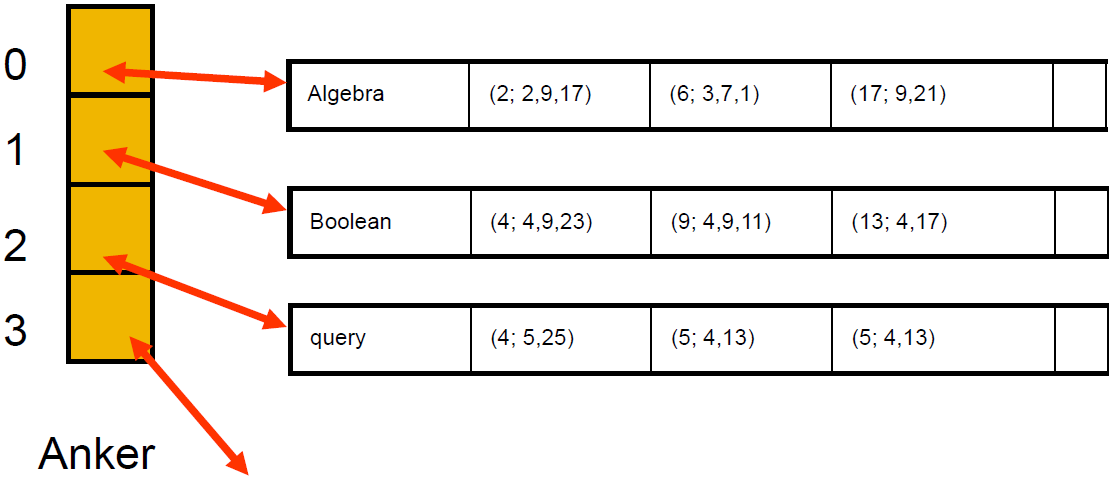
\includegraphics[width=150px]{img/HashDatei.png}
        \captionof{figure}{Abbildung einer Hash-Datei}
        \label{fig:Abbildung einer Hash-Datei}
\end{Figure}

\textbf{Lösen von Kollisionen}
\begin{itemize}
   \item Lineare Methode: vermeiden den Adressraum der bereits besetzt ist
   \subitem Suche den nächst freien Adressraum, wo die Kollision auftrat
   \subitem Suchstrategie: Gehe zum nächsten freien Adressraum $\rightarrow$ verschiebe um eine fixe Anzahl von Adressen
   \subitem Ziel besteht immer darin die Merkmale für welche die Kollision auftraten, so nahe als möglich bei den ursprünglichen Hash-Adressen zu speichern 
   \item Verkettete Kollisionsdateien: Verknüpfe Dateien mit Zeigern
   \subitem Zeiger auf einen anderen freien Adressraum im Speicherplatz
   \subitem Stelle zusätzlichen Speicherplatz bereit für Kollisionsdateien
\end{itemize}

\section{MiniRetrieve}

\begin{Figure}
   \centering
    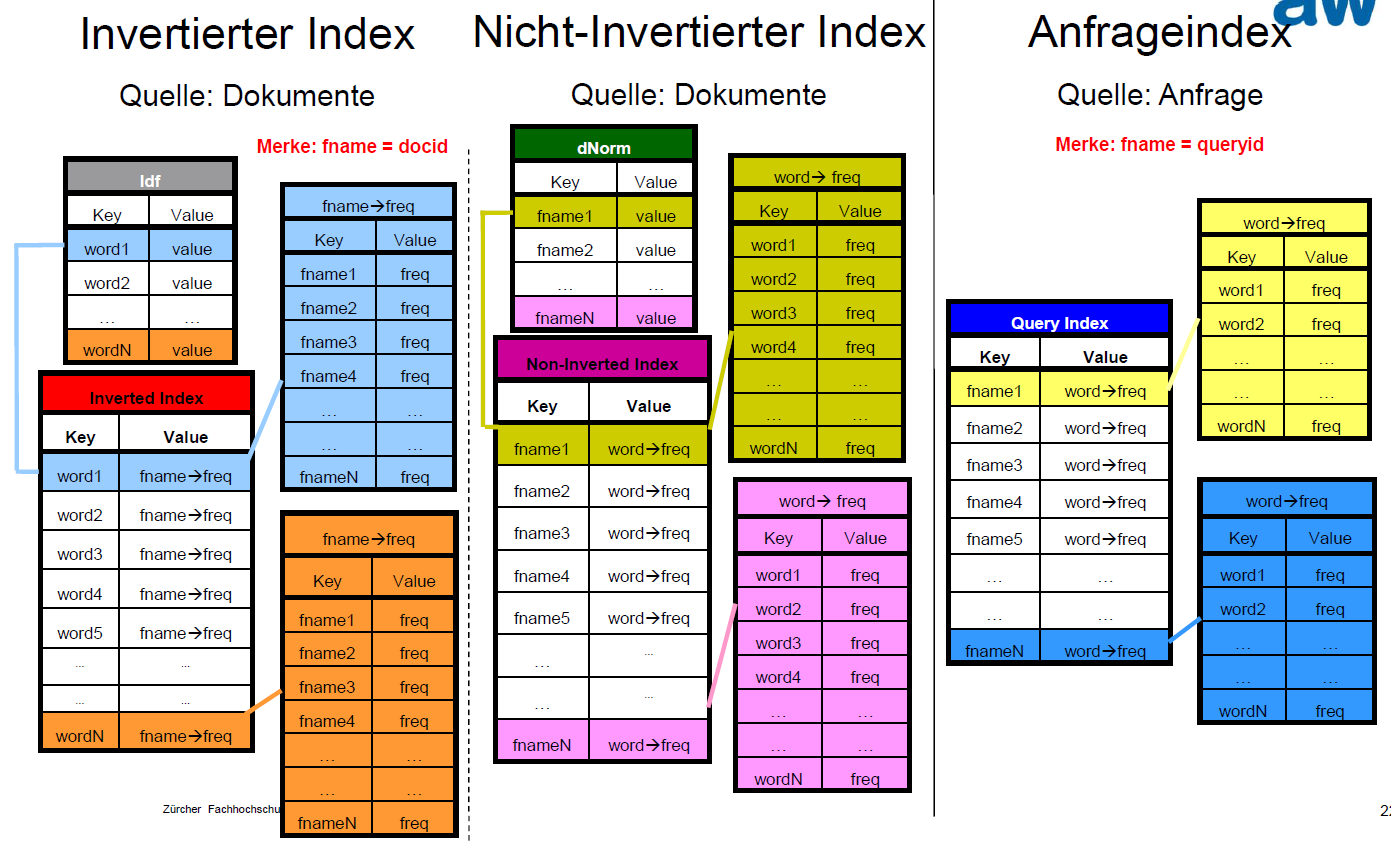
\includegraphics[width=150px]{img/ArchitekturMiniRetrieve.png}
        \captionof{figure}{Abbildung der Architektur des Mini Retrieves}
        \label{fig:Abbildung der Architektur des Mini Retrieves}
\end{Figure}

\chapter{Evaluation}

\section{Warum sollte man Information Retrieval Systeme evaluieren?}

IR Systeme unterscheiden sich grundsätzlich in ihren Grunddimensionen

\begin{itemize}
   \item Was sind die Dokumente/Informationen, welche erschlossen werden?
   \item Was sind die Paradigmen des Zugriffs (Pull, Push, Katalog)?
   \item Was sind die Benutzerkategorien, welche angesprochen werden?
   \item Was sind die Bedürfniskategorien, welche befriedigt werden müssen?
   \item Was ist das Geschäftsmodell?
\end{itemize}

$\rightarrow$ Daher muss evaluiert werden, ob die richtige Suchtechnologie am richtigen Ort eingesetzt wird

\begin{itemize}
   \item Evaluation ist notwendig, um die Leistung des Systems zu bewerten
   \item Da Information kein 'greifbares Gut' ist, ist eine Kosten/Nutzen-Analyse nur schwer zu erstellen
   \item Es ist schwierig, den Anteil der einzelnen Komponenten (Faktoren) an einem positiven oder negativen Suchresultat zu ermitteln (Datenabdeckung, Dateneinteilung, Anfrageformulierung, \dots)
   \subitem Wie gut ist das System?
   \subitem Wie gut könnte ein generisches System gleicher Bauart sein?
   \subitem Wie gut wäre ein optimales System?
   \subitem $\rightarrow$ wird das richtige System eingesetzt? 
\end{itemize}

\textbf{Achtung:} Es ist schwierig, aus vergangener Leistung auf zukünftige Leistung zu schliessen


\section{Zutaten einer Evaluation}

\subsection{1. Aufgabenstellung}
Eine seriöse Evaluation setzt eine klare Aufgabenstellung voraus:
\begin{itemize}
   \item Was sind die Motivation, Ziele und Vorgehensweise der Evaluation?
   \item welches sind die an den Resultaten interessierten Parteien?
   \item Wird eine 'interne' oder 'externe' Evaluation angestrebt?
   \item Ist das Vorgehen 'investigativ' oder wird 'experimentell' gearbeitet?
   \item Wird das System als 'blackbox' oder als 'glass box' behandelt?
   \item Was ist der Richtwert (Benchmark)? und andere Massstäbe
   \item Wird erschöpfend oder indikativ analysiert?
   \item Werden qualitative oder quantitative Kriterien untersucht?
\end{itemize}

\subsection{2. Ausgestaltung der Evaluation}
Es folgt das 'Design' der Evaluation, welche der Aufgabenstellung gerecht werden muss:
\begin{itemize}
   \item Was sind Leistungsfaktoren?
   \item Was sind die Leistungsmassstäbe?
   \item Was sind die Leistungsmasse?
   \item Was sind die Daten?
   \item Wie ist das Prozedere zu gestalten?
\end{itemize}

\subsection{3. Testdaten}
Für die Evaluation eines IR-Systems werden in der Regel Testdaten gebraucht. 
\begin{itemize}
   \item Daten über die Benutzer
   \item Daten über Informationsbedürfnisse
   \item Dokumentdaten
   \item Daten über die Relevanz der Dokumente in Hinsicht auf die Informationsbedürfnisse
\end{itemize}


\section{Das Cranfield Paradigma}
Ist das meistverbreitete Paradigma in akademischen Kreisen. Dabei gibt es drei Stufen der Evaluation der Retrievaleffektivität
\begin{itemize}
   \item Ganzer Wissensbeschaffungsprozess
   \item Ganzes Retrieval-System
   \item Komponenten des Retrievalsystems
\end{itemize}

\subsection{Aufgabenstellung}
\begin{itemize}
   \item zu evaluieren ist die Retrievaleffektivität des IR-Systems, mittels geeigneter Masse
   \item Es wird eine interne, direkte Evaluation angestrebt, d.h. die Effektivität soll direkt gemessen werden und nicht über ihren Anteil an einem grösseren Resultat, d.h. der IR-Lösung bewertet werden
   \item Die Evaluation soll experimentell erfolgen
   \item Das System wird als Blackbox behandelt
   \item erfolgt im Vergleich zu einem vorgegeben Richtresultat
   \item quantitative Evaluation
\end{itemize}

\subsection{Ausgestaltung (Design)}
Wird ein Labortest verwendet

\subsection{Ausbeute / Präzision}

\begin{itemize}
   \item Zwei allgemein anerkannte Masse für Retrievalqualität sind Ausbeute und Präzision
   \item Diese Eigenschaften dieser Masse sind gut analysiert und verstanden
   \item beide Masse modellieren die Annahme, dass möglichst viel relevante und möglichst wenig irrelevante Information gefunden werden soll
   \subitem Präzision: wenig irrelevante Information
   \subitem Ausbeute: möglichst viele relevante Information 
   \item Ziel: Optimierung eines oder beider Kriterien
   \item Die beiden Masse sind mengenbasiert
   \item Die Masse widersprechend sich
   \subitem hohe Ausbeute $\rightarrow$ niedrige Präzision
   \subitem hohe Präzision $\rightarrow$ niedrige Ausbeute 
\end{itemize}

\begin{equation}
   \begin{split}
      \text{Präzision} :=& \frac{\text{Anzahl relevante Dokumente im Resultat}}{\text{Anzahl Dokumente im Resultat}} \\
      \text{Ausbeute} :=& \frac{\text{Anzahl relevante Dokumente im Resultat}}{\text{relevante Dokumente in der Kollektion}}
   \end{split}
\end{equation}

\textit{Mathematische Definition}\\
Ausbeute: $P_r(q) := \frac{|D^{rel}_r (q)|}{|D^{rel} (q)|}$ \\
Präzision: $\pi_r (q) :? \frac{|D^{rel}_r (q)|}{|D_r (q)|}$ \\
Interpolierte Ausbeute/Präzisionsfunktion: $\prod_q (p) := max \{ \pi_r (q) | p_r (q) \geq p \}$\\
Wobei:
\begin{itemize}
   \item $D^{rel}_r (q)$ $\rightarrow$ Relevante Dokumente in der Resultatmenge
   \item $D^{rel} (q)$ $\rightarrow$ Menge aller relevanter Dokumente
   \item $D_r (q)$ $\rightarrow$ Alle Dokumente  der Resultatmenge
\end{itemize}

\subsection{Average Precision}
\begin{itemize}
   \item Durchschnitt der Präzisionswerte an den Rängen aller relevanten Dokumente $\rightarrow$ non-interpolated
   \item Durchschnitt der Präzisionswerte für spezielle Ausbeutungsgrade $\rightarrow$ interpolated
   \item Beliebteste \textit{Ein-Zahl-Mass}
\end{itemize}

\subsubsection{Mean Average Precision}

tbd - Kapitel 4 Slide 18

\subsubsection{Einschränkungen unserers Vorgehens}
\begin{itemize}
   \item Nur eine Anfrage
   \item Präzisionsorientiertes Szenario
   \item Können Ausbeute nicht bestimmen
   \item Datenbasis nicht eingefroren
   \item Datenbasis nicht identisch
   \item Wie sind die Relevanzbeurteilungen zu betrachten?
\end{itemize}

\subsubsection{Problem der Relevanzbewertung}


\chapter{Kategorisierung}

\section{Dokumentkategorisierung}
\textbf{Definition:} \textit{Bei der Kategorisierung werden Dokumente anhand ihres Inhaltes einer speziellen Kategorie zugewiesen}
\begin{itemize}
   \item Eine Kategorie sollte innerhalb einer bestimmten Domäne einen wohl definierten Bereich darstellen
   \subitem Es geht um den Umgang mit Bedeutung, obwohl wir in den meisten Fällen nur 'rohe Daten' zur Verfügung haben 
   \item Kategorien sind unter anderem in folgenden Fällen einen Mehrwert
   \subitem (Manuelle) Indexierung
   \subitem Suche nach Information in Dokumentenarchiven oder News Feeds
   \subitem Recommender (Netflix, Spotify etc) 
\end{itemize}

\subsection{Kategorisierung Aufgaben}
Es gibt eine Menge unterschiedlicher Aufgaben
\begin{itemize}
   \item Indexierung (Verschlagwortung)
   \subitem Manuelle Methode $\rightarrow$ schwerfällig und kostenintensiv
   \subitem Bei Automatischer Vergaben hat man ein kontrolliertes Vokabular 
   \item Recommender (klassisch: Routing / FIltering)
   \subitem Ein Userprofil bzw. Themenprofil wird regelmässig gegen die einkommenden Dokumente getestet, um zu bestimmen, wo letztere einzuordnen sind $\rightarrow$ verwandt: Push-Dienste
   \item Clustering
   \subitem Gruppieren von Kollektionen in eine Menge von sich gegenseitig ausschliessende Kategorien - die aus den Daten gebildet werden 
   \item Annotation 
   \subitem Gruppieren von Dokumenten mit weiterführender, dazugehöriger Information 
\end{itemize}

\subsubsection{Kategorisierung vs. Klassifikation}

Klassifikation: Man ist nur bei einem zugehörig

Kategorisierung: hat mehrere 'Tags'

offizielle Unterscheidung ergänzen

\section{Verfahren}

\subsection{Rocchio Model}
tbd

\subsection{kNN}
tbd

\subsection{Bayes Klassifizierung}
\begin{itemize}
   \item \textit{gegeben:} Kategorie $C_i$ mit einer angemessenen Anzahl von bereits zugeordneten Objekten (Trainingsdaten)
   \item \textit{Methode:} Bilde statische Modelle aus diesen Kategorien. Benutze diese, um vorherzusagen, zu welcher Klasse ein neues Objekt gehört
   \item Wir kennen $P(t|C_i)$ für alle $t|C_i$, sind aber eigentlich interessiert an: $P(C_i|t)$ oder noch spezifischer in $P(C_i|D)$
   \item Aus alten Objekten kann man bestimmen nach welchen Merkmale zu suchen ist 
   \item Annahme: Alle Dokumente sind voneinander unabhängig
\end{itemize}

\subsection{Collaborative Filtering}
Das collaborative filtering kann implizite und abstrakte Beziehungen zwischen zwei Filmen herstellen. \\
Beispielsweise: \textit{Ist Jason Statham ein ähnlicher Schauspieler wie Vin Diesel?} $\rightarrow$ bei kollaborativen Filtering ist die Aussage \textit{"Leute die A mögen, mögen auch B"}\\
\textbf{Achtung: } \textit{Ähnlichkeit bedeutet nicht notwendigerweise gleicher Geschmack}

\subsection{Thesaurus}
tbd

\begin{itemize}
   \item Aufpassen bei den Thesaurus muss man bspw. bei Synonymen, da es hier zu nicht korrekten Synonymen im Kontext kommen kann
\end{itemize}

\subsection{Herausforderungen bzgl Klassifikationen}
\begin{itemize}
   \item Aufwand für Verwaltung, wie erfasst man Unschärfe
   \item Vollständigkeit
   \item Bedeutungen ändern sich $\rightarrow$ Eine Klassifikation muss sich ändern können, das hat grossen Einfluss auf die Verwaltung von Klassifikationen
   \item Menschen klassifizieren unterschiedlich $\rightarrow$ ebenfalls abhängig von der Zeit
\end{itemize}

\section{Clustering}
\textbf{Definition:} \textit{Clustering ist ein Gruppierungsprozess bei dem eine Menge von Objekten in 'Cluster' von ähnlichen Objekten geordnet werden}



\chapter{Web-Suche}

\section{Suche im Web}
\begin{itemize}
   \item Korpus: Das öffentliche zugreifbare Web besteht aus statischem und dynamischen Inhalt
   \subitem Daten im Web sind unbeständig $\rightarrow$ 40\% monatliche Änderung, unstrukturiert, teilweise schlechte Qualität und/oder heterogen
   \item Wird verwenden um sich zu navigieren
   \item Ziel: Finde qualitativ hochstehende Resultate (nicht zwingend Dokument), die für den Benutzer relevant sind
   \subitem Statische Seiten
   \subitem Resultate sind nicht ausbeuteorientiert
   \item Bedürfnisse
   \subitem informationell
   \subitem navigational
   \subitem transaktional
   \subitem graubereiche
   \item Soll nicht überschätzt werden
\end{itemize}

\subsection{Anatomie von Suchmaschinen}
\begin{itemize}
   \item Spider (Crawler oder Roboter) - bildet den Korpus
   \subitem Sammelt die Daten rekursiv
   \subsubitem Für jede bekannte URL, hole die WEbseiten, parse diese und extrahiere die neuen URLs
   \subitem Zusätzliche Daten von direkten Einträgen und anderen Quellen
   \subitem Verschiedene Suchmaschinen haben unterschiedliche Grundsätze - kleine Übereinstimmung unter den Korpora 
   \item Der Indexer - verarbeitet die DAten (inverted files)
   \subitem Verschiedene Grundsätze, welche Worte indexiert oder gestemmt werden, Phrasenunterstützung, Grossschreibung, UniCodeUnterstützung etc. 
   \item Anfrageverarbeitung - akzeptiere Anfrage und liefere Resultate 
\end{itemize}

\subsubsection{Spidering}
\begin{itemize}
   \item Starte mit einer umfassenden Menge von URLs, von welchen die Suche (Spidering) gestartet wird (Seeds S0)
   \item Speichere die Dokumente in D und die Hyperlinks in E. Dabei ist sowohl D als auch E ein eigenständiger Datenbehälter
   \item Während dem Crawling wird eine Liste Q von URLs intern unterhalten
   \item Wir extrahieren evtl. eine URL von Q oder fügen eine URL Q hinzu
   \subitem Funktion: Dequeue() und Enqueue()
   \item Bezeichnungen
   \subitem u, v als eine URL
   \subitem d(u) die zugehörige Webseiten  
\end{itemize}

\textbf{Anker}
\begin{itemize}
   \item extrahiere Ankertexte (zwischen <a> und </a>) für jeden Outlink)
   \item Normalerweise beschreibt der Ankertext das DOkument sehr gut, auf welches es zeigt
   \item Füge Ankertext hinzu, damit die Zielwebseite mit zusätzlichen Schlüsselwörter versehen wird
   \item Sehr effektiv, um relevante Information zu finden
   \item Google bietet teilweise Suchresultate, die nur aufgrund des Ankertexts zustande gekommen ist
\end{itemize}

\section{Indexierung Webseiten}
\begin{itemize}
   \item Die exakte Indexierungsstrategie ist ein Geschäftsgeheimnis und variiert von Unternehmung zu Unternehmung
   \item Extremfall: Mann kann die Beschreibung jeder Seite auf die Kollektion der zugehörigen Ankertexte beschränken
   \item SPAM ist ein Problem, sowohl beim Spidern, als auch beim Indizieren
\end{itemize}

\subsection{Anfrageverarbeitung}
\begin{itemize}
   \item Google verarbeitet ca. 5 Mrd. Anfragen pro Tag
   \item kleine Anzahl von häufigen Anfragen (80/20 Regeln) $\rightarrow$ aktuell bspw. Corona
   \item nächste Resultatseite vorberechnen
   \item Falls die Anfrage gesucht werden muss $\rightarrow$ cluster von PCs
\end{itemize}

\section{Suchmaschinen Schlussfolgerung}
\begin{itemize}
   \item Spidering ist ein wichtiger Aspekt (was nicht im INdex ist, kann nicht gefunden werden)
   \item Ranking ist der Schlüssel (eine gute Antwort in den Top 5/10)
   \item Verwendung von verschiedene Merkmalen $\rightarrow$ präzisionsorientiert
   \item Stemming / Stoppwortliste verbessert nicht immer das Resultat im gewünschten Sinne
   \item Geschwindigkeit und Wirtschaftlichkeit ist ein Schlüsselelement
\end{itemize}

$\Rightarrow$ Je mehr Daten desto, einfacher ist die Suche

\section{Suche und Hyperlink}

\subsection{Spreading Activation (SA)}
\begin{itemize}
   \item Das WWW wird als Hypertext verstanden
   \item tbd
\end{itemize}

\subsection{Indegree}
\begin{itemize}
   \item Indegree ist die Anzahl der einkommenden Links zu einem gegebenen Dokument
   \item Indegree als Qualitätseinflussfaktor ist schwach
   \item tbd
\end{itemize}

\subsection{PageRank}
\begin{itemize}
   \item Zu Beginn ist der Surfer auf einer zufälligen Webseiten
   \item PageRank einer Webseite = Wahrscheinlichkeit, dass ein Surfer sich zu einem beliebigen Zeitpunkt auf dieser Webseite befindet
\end{itemize}

\textbf{Gedanken zu PageRank}
\begin{itemize}
   \item Berechnung rekursiv
   \item Kann offline berechnet werden
   \item Anfangs Page-Rank aller Knoten = 1
   \item Konvergiert gegen "Random-Surfer"-Wahrscheinlichkeiten
   \item Durchaus anfällig auf Spam
\end{itemize}

\subsection{Kleinberg Model}
\begin{itemize}
   \item HITS (Hypertext Induced Topic Selection) vorgeschlagen von Kleinberg
   \item Eine Webseite kann angesehen werden als
   \subitem Ein Hub (Zeigt auf gute Quellen)
   \subitem Eine Autorität (besitzt den Inhalt)
   \item Von einer Ursprungsmenge R, ziehen wir alle Nachbarn in Betracht
   \item Von dieser erweiterten Menge können wir die 'hubness' und autorität jedes einzelnen KNotens 
\end{itemize}

\end{document}